%% tex/recursivesets.tex
%% Copyright 2019 Andrea Berlingieri
%
% This work may be distributed and/or modified under the
% conditions of the LaTeX Project Public License, either version 1.3
% of this license or (at your option) any later version.
% The latest version of this license is in
%   http://www.latex-project.org/lppl.txt
% and version 1.3 or later is part of all distributions of LaTeX
% version 2005/12/01 or later.
%
% This work has the LPPL maintenance status `maintained'.
%
% The Current Maintainer of this work is Andrea Berlingieri.
%
% This work consists of all files listed in manifest.txt
\chapter{Insiemi ricorsivi e ricorsivamente enumerabili}

Supponiamo di voler trasmettere un insieme. Se questo è finito non c'è nessun problema, basta
mandare i suoi elementi. Se ho un insieme infinito posso trasmettere il programma che calcola la
funzione caratteristica del mio insieme. Non posso immaginare di poter trasmettere tutti gli insiemi
in questo modo, altrimenti potrei risolvere il problema della terminazione diagonale. Quelli per
cui è possibile sono detti ricorsivi.

% definition?
\begin{defn}
    Un insieme $A$ è ricorsivo sse $c_{A}$ è calcolabile.
\end{defn}

Un altro modo per trasmettere il mio insieme in maniera effettiva è dare un metodo di calcolo,
detto funzione enumerativa. Supponiamo di avere un insieme ${a_{0},a_{1},a_{2},\dotsc}.$ Diamo una
funzione $f$ tale che $f(0) = a_{0}$, $f(1) = a_{1}$, ecc. Abbiamo che $A = \cod(f)$.

Quando posso dare l'insieme in questa maniera ed $f$ è calcolabile si dice che l'insieme è
ricorsivamente enumerabile. Ricorsivamente è terminologia veccha, degli anni trenta del XX secolo.
In queste due accezioni ricorsivo va visto come sinonimo di calcolabile.

\begin{defn}
    $A$ è ricorsivamente enumerabile sse esiste una funzione di enumerazione $f$ per $A$
    calcolabile: $A = \cod(f)$, per $f$ calcolabile.
\end{defn}

\section{Relazione tra insiemi ricorsivi e r.e.}

Esistono quindi sostanzialmente due modi per descrivere in maniera effettiva un insieme $A$.
Vogliamo capire che relazione c'è tra queste due nozioni: qual è più potente? Come si rapportano?

Per descrivere una classe è spesso utile capire rispetto a quali operazioni la classe è chiusa. In
particolare, se $A$ è ricorsivo cosa possiamo dire del complementare di $A$, o
dell'unione/intersezione/differenza di $A$ con un altro insieme ricorsivo?

Ricordiamo che $A \subseteq \Nat$. Abbiamo che:
\begin{itemize}
    \item $\emptyset$ è ricorsivo: la funzione costante $\bm{0}$ è calcolabile;
    \item $\Nat$ è ricorsivo: la funzione costante $\bm{1}$ è calcolabile;
    \item ogni insieme finito è ricorsivo: $D$ è finito $\implies$ $D$ è ricorsivo:
    \begin{equation*}
        c_{D}(x) = 
        \begin{cases}
            1 \quad & \text{se $x = d_{1} \lor x = d_{2} \lor \dotsc \lor x = d_{n}$}  \\
            0 \quad & \text{altrimenti}
        \end{cases}
    \end{equation*}
    Sarebbe esprimibile anche con una serie di \textit{if}. Qualunque sia $D$ ho un modo per scrivere la mia
    funzione caratteristica.
\end{itemize}

Con lo stesso ragionamento posso dimostrare che molte altre funzioni sono calcolabili. Ad esempio
una funzione con \textit{Range} finito è sicuramente calcolabile; è scrivibile con un \textit{case}
ad esempio.  Tutte le funzioni scrivibili con un \textit{case} sono sicuramente calcolabili. Queste
funzioni hanno sempre un numero finito di elementi su cui hanno un comportamento interessante e nei
restanti hanno lo stesso comportamento.

L'insieme dei numeri pari è ricorsivo. Tutti gli insiemi primitivi ricorsivi, ovvero con funzione
caratteristica primitiva ricorsiva, sono sicuramente ricorsivi. Infatti le funzioni primitive
ricorsive sono un caso particolare di algoritmo.

Esistono insiemi non ricorsivi. Ad esempio $K = \{i \mid \phii(i) \converges\}$ non è ricorsivo.

Supponiamo che $A$,$B$ siano ricorsivi. Abbiamo che:
\begin{itemize}
    \item $\comp{A}$ è ricorsivo. Questo perche $c_{\comp{A}}(x) = 1 - c_{A}(x)$
    \item $A \cup B$ è ricorsivo. Questo perche $c_{A \cup B}(x) = \max(c_{A}(x),c_{B}(x))$
    \item $A \cap B$ è ricorsivo. Questo perche $c_{A \cap B}(x) = \min(c_{A}(x),c_{B}(x))$
\end{itemize}

Gli insiemi ricorsivi formano un'algebra di Boole, essendo chiusi per queste tre operazioni. Sono
una sottostruttura interessante degli insiemi.

Data una funzione caratteristica è facile costruire una funzione di enumerazione. In altri termini,
se un insieme è ricorsivo è anche ricorsivamente enumerabile. C'è un piccolo inghippo però a cui
bisogna fare attenzione.

La funzione di enumerazione potrebbe essere costruita nel seguente modo ad esempio:
% python snippet
\begin{python}
    def $e_{A}(i)$:
        $c$ = 0
        $j$ = 0
        while $c \leq i$:
            if $c_{A}(j)$:
                $c++$
            $j++$
        return $j-1$
\end{python}

In versione funzionale potremmo scrivere scrivere $e_{A}$ come $e_{A}(i+1) = \mu j, c_{A}(j) = 1
\land j > e_{A}(i)$, con $e_{A}(0) = \mu j, c_{A}(j) = 1$. Il piccolo dettaglio a cui fare
attenzione è che la funzione di enumerazione la vorremmo totale e calcolabile. Tuttavia questo non è
un vincolo così restringente.

Diamo la seguente definizione: $A$ è r.e. se esiste $f$ totale calcolabile tale che $A = \cod(f)$
oppure $A$ è vuoto.

Il problema della nostra funzione di enumerazione è che può divergere con insiemi finiti. Se, ad
esempio, ho un $A$ con 7 elementi e cerco l'ottavo con la mia funzione avrò che divergerà.

Il teorema rimane, se $A$ è ricorsivo è ricorsivamente enumerabile. Bisogna giusto ricordarsi che
per gli insiemi finiti va fatto un caso speciale che gestisca input maggiori della cardinalità di
$A$.

Più precisamente, se $A$ è finito, con $A = {a_{0},\dotsc,a_{n}}$, allora definiamo $e_{A}$ nel
seguente modo:
\begin{equation*}
    e_{A}(x) = 
        \begin{cases}
                x = 0 \Rightarrow a_{0} \\
                x = 1 \Rightarrow a_{1} \\
                \vdots \\
                x = n \Rightarrow a_{n} \\
                \textit{default} \Rightarrow a_{n}
        \end{cases}
\end{equation*}

%Abbiamo che $A$ è ordinato rispetto all'ordinamento sui naturali. Di conseguenza le mie due funzioni
%sono monotone crescenti (seguiamo l'ordine) e possiamo ordinare l'insieme in maniera almeno non
%decrescente (strettamente crescente nel caso di insiemi finiti).

Abbiamo quindi che Ricorsivo $\implies$ R.E. Vale il viceversa? La risposta è no, ma non è del tutto
ovvia.

Sia $A$ un insieme r.e. Potremmo pensare di calcolare la funzione caratteristica di $A$ con la sua
funzione di enumerazione, nel seguente modo:
\begin{python}
    def $c_{A}(x)$:
        $i$ = 0
        while $e_{A}(i) \not= x$:
            $i++$ 
        return 1
\end{python}

Questa $c_{A}$ però non calcola la funzione caratteristica di $A$, bensì la funzione
semicaratteristica di A,che indicheremo con $s_{A}$.
\begin{equation*}
    s_{A}(x) =
    \begin{cases}
        \case{1}{se $x \in A$} \\
        \case{\diverges}{altrimenti}
    \end{cases}
\end{equation*}

Questa funzione è calcolabile e parziale. Per ora abbiamo dimostrato che la funzione
semicaratteristica di $A$ è calcolabile, non abbiamo ancora dimostrato che r.e. $\centernot\implies$
ricorsivo. Dobbiamo mostrare un esempio di insieme r.e. che non sia ricorsivo. $K$ è non
ricorsivo. $K$ è r.e.?

Proviamo a scrivere una funzione di enumerazione per $K$:
\begin{python}
    def $e_{K}(\pair{i}{t})$:
        if $T^{3}(i,i,t) = 1$:
            return i
        else:
            return $k_{0}$
\end{python}
        
Nell'else è importante che restituisca un programma che sta in $K$. Ce ne sono tanti e di semplici;
ad esempio le funzioni costanti. Diamo indice $k_{0}$ ad un tale programma.

È una buona funzione di numerazione? È sicuramente calcolabile. È suriettiva? È facile vedere che
numero solo cose che stanno in $K$: $k_{0}$ sta in $K$ e se restituisco $i$ allora $i$ stava in $K$.
Se $i$ sta in $K$ vuol dire che esiste un $t$ tale che $\phii \converges$ in $t$ passi. Di conseguenza
vengono enumerate tutte le funzioni convergenti su $i$ di indice $i$. 

Il dovetailing è al variare dell'input. Mi muovo sugli input e sul tempo di computazione.

Si potrebbe fare anche nel seguente modo:
\begin{equation*}
    e_{K}(c) = fst(\mu \pair{i}{t}, \pair{i}{t} \geq c \land T(i,i,t))
\end{equation*}

Il risultato finale è che $K$ è ricorsivamente enumerabile.

C'è un'altra relazione notevole tra insiemi r.e. e insiemi ricorsivi.

\begin{thm}
    Sia $A$ un insieme tale che sia $A$ che $\comp{A}$ sono r.e. Allora $A$ è ricorsivo.
\end{thm}
\begin{proof}
    Supponiamo di aver $e_{A}$ ed $e_{\comp{A}}$. Informalmente, possiamo far partire la ricerca per
    entrambe le funzioni. Prima o poi una terminerà, e in base a quale termina ho la mia risposta. La
    computazione parallela è assolutamente algoritmica e non c'è problema al riguardo.

    Più formalmente, sia $h$ così definita:
    \begin{equation*}
        h(x) =
        \begin{cases}
            \case{e_{A}(x)}{se $x = 2n$ per qualche $n$} \\
            \case{e_{\comp{A}}(x)}{se $x = 2n+1$ per qualche $n$} \\
        \end{cases}
    \end{equation*}
    Possiamo scrivere $c_{A}(n) = \textit{pari}(\mu i, h(i) = n)$
\end{proof}

Come corollario di questo teorema abbiamo che esiste un insieme nè ricorsivo nè r.e. Quale?
$\comp{K}$. Se infatti $\comp{K}$ fosse r.e. allora $K$ sarebbe ricorsivo.

Abbiamo una gerarchia degli insiemi fatta in questo modo: 

\begin{figure}[h]
    \centering
    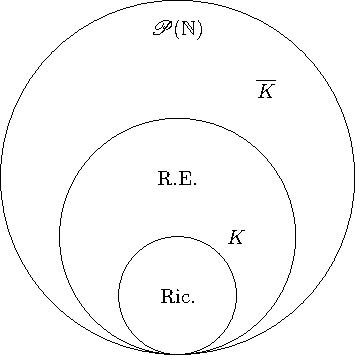
\includegraphics{./img/recursivesets/RecursiveHierarchy.pdf}
    \caption{Gerarchia degli insiemi r.e. e ricorsivi}
\end{figure}

\newpage

\section{Enumerazioni iniettive e monotone}

Ci concentriamo ora sulle proprietà dell'enumerazione. Ci chiediamo in particolare cosa possiamo
dire riguardo alla sua monotonia e alla sua iniettività.

Supponiamo di poter enumerare $A$ con una funzione effettiva. Ci chiediamo se possiamo trasformare
$f$ in modo da non avere ripetizioni. Se pensiamo all'enumerazione come ad uno stream infinito di
numeri in input ci chiediamo se possiamo creare un filtro che elimini i duplicati dallo stream.

Questo si può fare in maniera algoritmica tenendo una lista dei numeri ricevuti dallo stream e, ogni
volta che ho un nuovo numero, controllo se è gia nella lista. In base al risultato decido se
aggiungerlo o meno alla lista. La mia lista è ora il mio nuovo stream senza ripetizioni. Abbiamo
quindi che non è restittivo richiedere che la mia enumrazione sia iniettiva.

Diamo quindi la seguente definizione:

\begin{defn}
    $A$ è R.E. sse $\exists f$ iniettiva tot. calc. tale che $A = \cod(f)$ oppure $A$ è finito.
\end{defn}

A livello formale data l'enumerazione $f$ possiamo costruire una nuova enumerazione $g$ per lo
stesso insieme che sia iniettiva nel seguente modo:
\begin{equation*}
    g(x) =
    \begin{cases}
        \case{f(0)}{se $x = 0$} \\
        \case{f(\mu i, \forall y \leq x-1, f(i) \not= g(y))}{altrimenti}
    \end{cases}
\end{equation*}

Questo ha senso per insiemi infiniti.

L'iniettività è quindi una proprietà accettabile per la mia enumerazione. Posso trasformarla anche
in una funzione monotona crescente? La risposta sarà no, non posso enumerare gli elementi di $A$ in
maniera crescente se $A$ è r.e.

Il problema è fondamentalmente che non posso assicurarmi che un dato elemento sia il più piccolo
nello stream. La ricerca divergerebbe. Ogni volta che cerchiamo un minimo c'è un problema del
genere.

L'idea è che se potessimo ordinare gli elementi di $A$ allora $A$ sarebbe ricorsivo. Dato che non tutti
gli insiemi r.e. sono ricorsivi non si può fare in generale.

Sia $f$ un'enumerazione strettamente crescente. Essendo discreta cresce strettamente più
dell'identità. Se voglio sapere se $x$ fa parte della mia numerazione posso controllare gli elementi
fino ad $x$, oltre sicuramente non lo troverò.

Più formalmente, la ricerca di $x$ può essere fatta col seguente algoritmo:
\begin{python}
    $i_{x}$ = $\mu i, f(i) \geq x$
    return ($f(i_{x}) == x$)
\end{python}

In questo modo sono sicuro, se $f$ è strettamente crescente, che la mia ricerca termina. Per capire
se $x$ stava nel mio stream controllo che $f(i_{x})$ sia uguale ad $x$. 

Questo algoritmo funziona se la mia funzione è non decrescente? Se la mia funzione diventa
indefinitamente costante da un certo punto in poi potrei andare avanti all'infinito. La mia
minimizzazione non ha più garanzia di terminare.

Questo problema sorge quando $\cod(f)$ è finito. Quando $\cod(f)$ è infinito prima o poi la funzione
assumerà un nuovo valore. Tuttavia se $\cod(f)$ è finito allora l'insieme enumerato da $f$ è
ricorsivo.

Ogni insieme ricorsivo infinito è enumerabile mediante una funzione di enumerazione crescente. Ogni
insieme ricorsivo non vuoto è enumerabile mediante una funzione di enumerazione non decrescente.

Se si è in grado di ordinare si è anche in grado di decidere. Gli approcci generativi sono
generalmente semidecidibili e permettono di generare elementi in maniera disordinata.

Riprendiamo ora $K = \{i \mid \phii(i) \converges\}$. Come decidiamo se un certo $i$ sta in $K$? Possiamo far
partire il mio interprete e aspettare. Se termina allora $i$ appartiene a $K.$ Se non appartiene a
$K$ non lo saprò mai, perché dovrei aspettare che il programma termini. Di $K$ non possiamo quindi calcolare
la funzione caratteristica, bensì la funzione semicaratteristica:
\begin{equation*}
    s_{K}(i) = 
    \begin{cases}
        \case{1}{se $\phii(i) \converges$} \\
        \case{\diverges}{altrimenti}
    \end{cases}
\end{equation*}

In generale la funzione semicaratteristica di $A$, con $A$ r.e., è fatta nel seguente modo:
\begin{equation*}
    s_{A}(x) = 
    \begin{cases}
        \case{\converges}{se $x \in A$} \\
        \case{\diverges}{se $x \notin A$}
    \end{cases}
\end{equation*}

In alcuni casi posso semidecidere la appartenenza di un elemento ad un insieme, in altri casi potrei
non esserne in grado.

\section{Insiemi r.e. e semidecisione}

Ci chiediamo ora che legame esista tra la capacità di enumerare e la capacità di semidecidere. Ce
lo chiediamo in generale, ricordando che per $K$ l'abbiamo già visto.

Supponiamo che $A$ sia vuoto oppure $A = \cod(f)$, con $f$ tot. calcolabile. Come faccio a costruire
l'algoritmo di semidecisione per $A$? Semplicemente comincio a cercare $x$ nell'enumerazione.
\begin{equation*}
    s_{A}(x) = (\mu i, (f(i) = x))
\end{equation*}

Come facciamo per il viceversa? Abbiamo la procedura di semidecisione per $A$ e vogliamo costruire la
funzione di enumerazione per $A$. $f$ è delicata perché potrebbe divergere. Dobbiamo essere più
astuti. L'idea è muoversi mediante dove tailing sull'input e sul tempo di computazione.
\begin{equation*}
    f(\pair{x}{t}) =
    \begin{cases}
        \case{x}{se $s_{A}(x)$ termina nel tempo $t$} \\
        \case{a_{0}}{altrimenti}
    \end{cases}
\end{equation*}

$f$ è totale e calcolabile. Abbiamo quindi un'enumerazione per $A$. Non è iniettiva, ma questo non
importa. $a_{0}$ è un elemento qualsiasi di $A$. Possiamo quindi vedere la semidecisione come
enumerazione di un insieme r.e. e viceversa.

Non siamo sicuri di poter trovare $a_{0}$. Questo pezzo della dimostrazione è non costruttivo. Dal
punto di vista classico però o l'insieme è vuoto, e quindi r.e., oppure non lo è e deve avere almeno
un elemento $a_{0}$. Deve quindi esistere la funzione calcolabile $f$, anche se non è detto che
possiamo trovarla.

Vediamo ora un'applicazione. Quali sono le proprietà di chiusura per gli insiemi r.e.? Sono chiusi
per complementazione? No, altrimenti gli insiemi r.e. sarebbero tutti ricorsivi, e sappiamo che
questo non è vero. Ad esempio $K$ è r.e. e $\comp{K}$ non lo è.

Cosa possiamo dire di $A \cup B$ e $A \cap B$? Per $A \cup B$ è abbastanza ovvio. Dati $f_{A}$ e
$f_{B}$ possiamo costruire $f_{A \cup B}$ in modo che $f_{A \cup B}(2x) = f_{A}(x)$ e $f_{A \cup
B}(2x + 1) = f_{B}(x)$. Per $A \cap B$ è semplice costruire il semidecisore di $A \cap B$ dati
quelli per $A$ e per $B$. Basta concatenare i due: $s_{A \cap B}(x) = s_{A}(x);s_{B}(x)$.

Piccola nota sulla notazione. Noi consideriamo funzioni parziali da $\Nat$ a $\Nat$: $f: \Nat
\partialto \Nat$. Indichiamo, in maniera impropria, $\cod(f) = \{y \mid \exists x, y = f(x)\}$ e
$\dom(f) = \{x \mid f(x) \converges\}$. Il nostro codominio in realtà è il \textit{Range} della
funzione ed il nostro dominio è il dominio di congergenza (o co-\textit{Range}). In termini del grafo abbiamo che $\dom(f)
= \{x \mid \exists y, \pair{x}{y} \in \textit{grafo}(f)\}$.

\section{Caratterizzazioni alternative di un insieme r.e.}

Vediamo ora alcune caratterizzazioni, tutte equivalenti, degli insiemi r.e. che sono più adatte in
certi contesti.

Se si può caratterizzare un insieme r.e. $A$ come il dominio di convergenza di una funzione $s$ abbiamo
che $s$ rappresenta la funzione di semidecisione di $A$.

Abbiamo visto che $A$ è r.e. sse $A = \emptyset \lor A = \cod(f)$, $f$ tot. calc.

Abbiamo però che $A$ può essere visto come $\dom(g)$, con $g$ parz. calc. È una definizione
equivalente a quella appena citata.

Si può infine definire $A$ anche come $A = \cod(h)$, con $h$ parz. calc.

Solitamente quando costruiamo una funzione di enumerazione la vogliamo totale, è meno problematica.

Le tre definizioni sono equivalenti appena viste sono equivalenti. 

\begin{thm}
    Le tre seguenti affermazioni sono equivalenti e definiscono tutte un insieme r.e. $A$:
    \begin{enumerate}
        \item \label{re1} $A = \emptyset \lor A = \cod(f)$, con $f$ totale calcolabile \\
        \item \label{re2} $A = \dom(g)$, con $g$ parziale calcolabile \\
        \item \label{re3} $A = \cod(h)$, con $h$  parziale calcolabile
    \end{enumerate}
\end{thm}
\begin{proof}
    Lo dimostriamo facendo vedere che $\eqref{re1} \implies \eqref{re2}$, $\eqref{re2} \implies
    \eqref{re3}$ e $\eqref{re3} \implies \eqref{re1}$.

    \begin{itemize}
        \item $\eqref{re1} \implies \eqref{re2}$:

        Se $A = \emptyset$, allora abbiamo che $A = \dom(f_{\emptyset})$, se indichiamo con
        $f_{\emptyset}$ la funzione ovunque divergente.

        Se invece $A \not= \emptyset$ sia $f$ tale che $A = \cod(f)$. Definiamo $g$ come
        \begin{equation*}
            g(x) = \mu y, f(y) = x
        \end{equation*}
        
        Si ha che $A = \dom(g)$.

        \item $\eqref{re2} \implies \eqref{re3}$:

        Sia $A = \dom(g)$, con $g$ parziale calcolabile. Sia $h$ la funzione calcolata dal seguente
        programma:
        \begin{python}
            def $h(x)$:
                $g(x)$ 
                return $x$ 
        \end{python}
        Se $g(x)$ termina restituisco $x$. Si ha che $A = \cod(h)$.

        \item $\eqref{re3} \implies \eqref{re1}$: 
        
        Abbiamo due casi: $A$ è vuoto oppure no.

        Se $A = \emptyset$ l'asserto è già dimostrato.

        Se $A \not= \emptyset$ allora $\exists a \in A$. A questo punto definisco la mia $f$ come:
        \begin{equation*}
            f(\pair{x}{t}) = 
            \begin{cases}
                \case{h(x)}{se $h(x)$ termina entro il tempo $t$}\\
                \case{a}{altrimenti}
            \end{cases}
        \end{equation*}

        $f$ è totale, perché do sempre in output un valore. È calcolabile, sotto l'ipotesi che $h$
        sia calcolabile. Infine $\cod(f) = A$ perché $f$ restituisce solo elementi in $A$ e me li
        restituisce tutti, dato che $A = \cod(h)$.
    \end{itemize}
\end{proof}


La definizione \eqref{re3} ci permette di non doverci soffermare sul caso particolare dell'insieme
vuoto, che non ha implicazioni tecniche importanti.

\subsection{Teorema della proiezione}

Un'ulteriore caratterizzazione degli insiemi r.e. è la seguente:

\begin{thm}
    $A$ è r.e. sse $\exists B$ ricorsivo tale che $A = \{x \mid \exists y, \pair{x}{y} \in B\}$.
\end{thm}
\begin{proof}
    Vediamo i due versi del $\iff$ separatamente:
    \begin{itemize}
        \item $\implies$ Sia $c_{B}$ la funzione caratteristica di $B$. Allora $A = \dom(f)$, con
        \begin{equation*}
            f(m) = \mu n, c_{B}(\pair{n}{m}) = 1
        \end{equation*}
        \item $\implied$ Sia $A = \dom(\phii)$. Quindi $m \in A$ sse $\phii(m) \converges$, ovvero
        se $\exists t, T^{3}(i,m,t) = 1$, dove $T$ è il predicato ternario di Kleene.
        Basta quindi porre:
        \begin{equation*}
            B = \set{\pair{m}{t} \mid \exists t, T^{3}(i,m,t)}
        \end{equation*}
    \end{itemize}
\end{proof}

Possiamo vedere $B$ come una codifica delle coppie oppure come un insieme di coppie, non è
importante.

$A$ è la proiezione esistenziale di $B$ 

\begin{figure}[h]
    \centering
    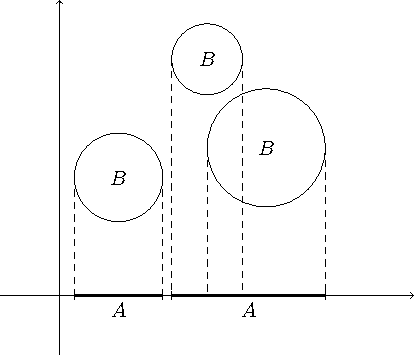
\includegraphics{./img/recursivesets/ExistentialProjection.pdf}
    \caption{Proiezione esitenziale di $B$}
\end{figure}

Il teorema è importante. Se ho un insieme ricorsivo e ne faccio la proiezione esistenziale ottengo
un insieme r.e. $x \in A$ sse $\exists y, (x,y) \in B$. Posso verificare se $(x,y)$ sta in $B$
perché $B$ è ricorsivo. Posso quindi semidecidere l'appartenenza di $x$ ad $A$ con un algoritmo del
genere ad esempio: $\mu y, (x,y) \in B$.

Se io faccio una ricerca in un dominio ricorsivo non è detto che questa termini. Se potessi dare dei
bound alla mia ricerca o avessi altre ipotesi potrei trasformare il mio algoritmo di semidecisione
in un algoritmo di decisione, ma in generale non è questo il caso. Avremo in generale una funzione
di semidecisione.

L'altra conseguenza importante è che qualunque problema semidecidibile può essere visto come una
ricerca in uno spazio decidibile.

È utile vedere $y$ come certificato di $x$, $c_{x}$. Il fatto che $x$ appartenga ad $A$ è cerficato da
$c_{x}$. Se $x \in A$ sappiamo che questo ceritificato esiste ma non sappiamo quale sia. La sua
ricerca non è però un problema decidibile.

Prendiamo per esempio la logica del prim'ordine. Se ho una formula in generale non è decidibile se
questa sia dimostrabile. Tuttavia abbiamo un algoritmo che genera tutte le formule dimostrabili nella
logica del prim'ordine. Dimostrare $F$ con questo algoritmo significa andare a cercare, nell'insieme
delle formule generate, un certificato per $F$. 

Un altro esempio è: dato un programma datemi un certificato per la sua appartenenza a $K$. Questo
certificato potrebbe essere il tempo $t$ in cui $\phi_{x}(x)$ termina. La dimostrazione che abbiamo
visto procede proprio in questo modo.

Il certificato non è un concetto ben definito, sta a noi decidere cosa sia un certificato. Un
certificato per un teorema potrebbe benissimo essere sia una prova che semplicemente la dimensione
della prova.

Ritorneremo su questo concetto quando parleremo di $\PClass$ e $\NPClass$. Vedremo che $\NPClass$ è l'insieme dei
linguaggi che sono proiezione esistenziale di un qualche linguaggio in $\PClass$. 

La caratterizzazione $A = \dom(\phii)$ è così importante che abbiamo della notazione specifica per
indicarlo: $W_{i}$. Possiamo con questa notazione definire $K$ come $K = \{i \mid i \in W_{i}\}$.
L'importanza di questa caratterizzazione è data dal fatto che essa induce una enumerazione di tutti
gli insieri r.e., basata sui domini di convergenza delle funzioni della mia enumerazione delle
funzioni calcolabili.

\section{Ulteriori proprietà di chiusura degli insiemi r.e.}

\begin{thm}
    Siano $A,B \subseteq \Nat$ e $f : \Nat \to \Nat$. Abbiamo che:
    \begin{enumerate}
        \item se $A$ è ricorsivo e $f$ è totale calcolabile, allora $f^{-1}(A)$ è ricorsivo
        \item se $A$ è r.e. e $f$ è calcolabile, allora $f^{-1}(A)$ è r.e.
        \item se $A$ è r.e. e $f$ è calcolabile, allora $f(A)$ è r.e.
    \end{enumerate}
\end{thm}
\begin{proof}
    Vediamo i tre punti uno per uno:
    \begin{enumerate}
        \item $c_{f^{-1}(A)}(x) = c_{A}(f(x))$
        \item Sia $A = \dom(g)$, con $g$ calcolabile. Consideriamo la seguente funzione:
        \begin{equation*}
            h(x) = g(f(x))
        \end{equation*}
        Questa funzione termina su $x$ sse $x \in \dom(f) \land f(x) \in \dom(g)$. Ma $\dom(g) = A$, quindi $h$ termina
        su tutti quegli $x$ tali che $f(x) \in A$. Ma quindi $f^{-1}(A) = \dom(h)$.
        \item Sia $A = \cod(g)$. Consideriamo la seguente funzione:
        \begin{equation*}
            h(x) = f(g(x))
        \end{equation*}
        Abbiamo che $\cod(h) = f(\cod(g))$. Ma $\cod(g) = A$, quindi $f(A) = \cod(h)$.
    \end{enumerate}
\end{proof}

Vediamo ora che le famiglie r.e. di insieme r.e. sono chiuse per unione ma non per intersezione. Per
farlo ci servirà l'enumerazione degli insiemi r.e. indotta dai domini delle funzioni calcolabili.
\begin{lem}
    Valgono le seguenti proprietà per gli insiemi r.e.:
    \begin{enumerate}
        \item $\forall x, \displaystyle\bigcup_{i \in W_{x}}W_{i}$ è r.e.;
        \item $\exists x, \displaystyle\bigcap_{i \in W_{x}}W_{i}$ non è r.e.;
    \end{enumerate}
\end{lem}
\begin{proof}
    Vediamo i due punti uno per uno:
    \begin{enumerate}
        \item possiamo scrivere il semidecisore di $\displaystyle\bigcup_{i \in W_{x}}W_{i}$ come
        segue, mediante dove-tailing:
        \begin{equation*}
            s_{\bigcup_{i \in W_{x}}W_{i}}(x) = \mu \pair{i}{t}, T(i,x,t)
        \end{equation*}
        \item 
        Sia $g$ la funzione così definita:
        \begin{equation*}
            g(i,x) =
            \begin{cases}
                \case{\diverges}{se $T(x,x,i)$} \\
                \case{0}{altrimenti} \\
            \end{cases}
        \end{equation*}
        Per s-m-n esiste $h$ totale calcolabile tale che:
        \begin{equation*}
            W_{h(i)} = \set{x \mid \lnot T(x,x,i)}
        \end{equation*}
        dove $T$ è il predicato ternario di Kleene. Si dimostra facilmente che:
        \begin{equation*}
            \bigcap_{i \in \Nat}W_{h(i)} = \comp{K}
        \end{equation*}
        Poichè $\displaystyle\bigcap_{i \in \Nat}W_{h(i)} = \displaystyle\bigcap_{i \in
        \cod(h)}W_{i}$ l'asserto risulta verificato.
    \end{enumerate}
\end{proof}

Ulteriore nota, nella seconda dimostrazione abbiamo che gli insiemi $W_{h(i)}$ sono ricorsivi e $h$
può essere scelta monotona crescente, quindi una intersezione ricorsiva di insiemi ricorsivi non è
in generale r.e.
